\subsection*{Genome Annotation}
\graphicspath{{../Rscript/CMG_Rscript_files/figure-gfm/}}

% * Genome annotation: what functions are encoded in your MAGs?
% Hypothetical/annotated proteins

Genome annotation was performed with \textit{Prokka}. Thanks to this tool the number of coding sequences (CDS), and non-coding sequences found within each genome were retrieved. CDS are divided in hypothetical and known proteins, while non-coding sequences are comprehensive of rRNAs, tRNAs, tmRNAs (bifunctional transfer-messenger RNAs) and repeat regions. Moreover, \textit{Prokka} provides the symbol for each known protein and its sequence length.

\begin{figure}[!h]
\centering
\begin{subfigure}{0.49\textwidth}
    \centering
    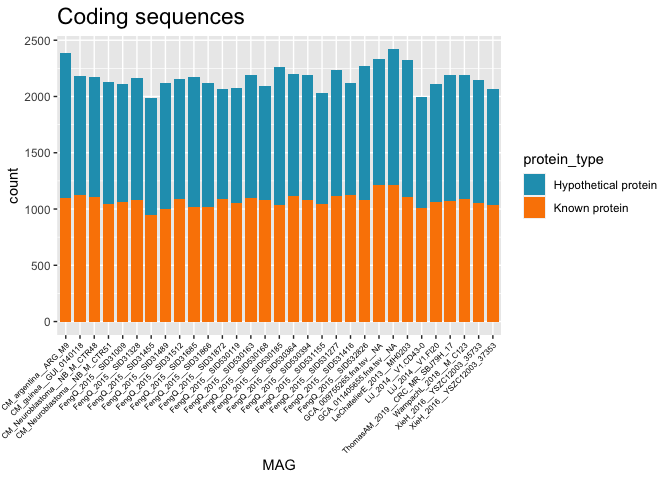
\includegraphics[width=\linewidth]{prokka_data-1.png}
    \caption{\footnotesize{\textbf{Number of coding sequences.} The number of coding sequences annotated for each MAG, divided in hypothetical and known proteins.}}
    \label{fig:prokka1}
\end{subfigure}
\begin{subfigure}{0.49\textwidth}
    \centering
    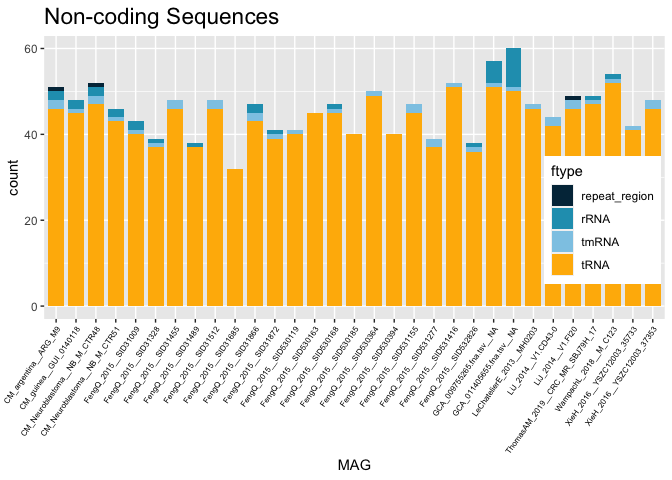
\includegraphics[width=\linewidth]{prokka_data-2.png}
    \caption{\footnotesize{\textbf{Number of non-coding sequences.} The number of non-coding sequences annotated for each MAG, divided in repeat regions, rRNAs, tmRNAs and tRNAs.}}
    \label{fig:prokka2}
\end{subfigure}
\caption{}
\end{figure}

The number of CDS in the set of MAGs goes to a minimum of 1988 to a maximum of 2544. For each genome, about half of the CDSs are non-characterized hypothetical proteins(Fig. \ref{fig:prokka1}). For what concerns non-coding sequences, the vast majority of them is represented by tRNAs (Fig. \ref{fig:prokka2}).